\documentclass[
hue = 206,
sdrawing = 0.44,
bdrawing = 0.73,
stext = 0.45,
btext = 0.44,
sline = 0.46,
bline = 0.15]{grigerart}

\title{Diario de Desarrollo}
\author{Gustavo Rivas-Gervilla}

\usepackage[spanish, es-tabla]{babel}

\usepackage{graphbox}
\usepackage[most]{tcolorbox}

\definecolor{noticeBg}{HTML}{eff4f8}

\tcbset{
  enhanced,
  sharp corners,
  frame hidden,
  borderline west = {0.5pt}{0pt}{black},
  colframe = black, colback = white,
  boxsep = 0pt, top = 0pt, bottom = 0pt
}

\newtcolorbox{notice}{
  overlay={\node[circle, align = center, text width = 5mm, inner sep=0pt, fill = white] at (frame.west) {
\includegraphics[height = 1em]{figures/megaphone.png}};}
}

\newtcolorbox{idea}{
  overlay={\node[circle, align = center, text width = 5mm, inner sep=0pt, fill = white] at (frame.west) {
\includegraphics[height = 1em]{figures/idea.png}};}
}

% commands
\newcommand{\issue}[1]{\href{https://github.com/Griger/REGwFCA/issues/#1}{\##1}}
\newcommand{\goal}[1]{\hyperref[sec:objetivos]{O#1}}

\newcommand{\entry}[1]{
    \begin{flushright}
      \textit{#1}
    \end{flushright}
}


% \renewcommand*\familydefault{\ttdefault}
% \usepackage[htt]{hyphenat}
%%% Local Variables:
%%% mode: latex
%%% TeX-master: "main"
%%% End:


\begin{document}
\maketitle
\tableofcontents

\section*{Bitácora \label{sec:bitacora}}
\addcontentsline{toc}{section}{Bitácora}

\entry{20/03/2020}

En el día de hoy vamos a trabajar en el objetivo \goal{1}, hemos de tener en cuenta que un retículo se puede almacenar en forma de grafo, ya que tenemos distintos nodos (los conceptos formales del contexto) que están relacionados entre sí en una jerarquía padre-hijo (que en nuestro caso vendrá dada por la relación de inclusión que se da entre conceptos formales). Así, en la Figura~\ref{fig:graph} tenemos un retículos en el que los conceptos han sido representados por medio de nodos en un grafo, donde podemos observar las distintas relaciones de inclusión que se dan entre los conceptos formales.

\begin{figure}[ht]
  \centering
  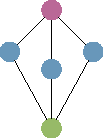
\includegraphics[]{figures/lattice.pdf}
  \caption{\label{fig:graph} Ejemplo de un retículo visto como un grafo donde podemos ver tres \textit{niveles} distintos de conceptos formales.}
\end{figure}

Esto da lugar al requisito r1 que es el primero que debemos afrontar de cara a desarrollar la base sobre la que se sustentará nuestra aplicación.

Así vamos a tener por un lado la clase \texttt{Lattice} que se encargará de soportar toda la estructura del retículo, y la clase \texttt{Node} que representará a cada uno de los nodos que conforman el retículo, es decir, cada uno de los nodos que podemos ver en la Figura~\ref{fig:graph}.

Además, queremos tener un acceso rápido a los conceptos de nuestro retículo, con lo cual lo que vamos a emplear será una tabla hash con la cual tener indexados nuestros conceptos formales, por medio de su \textit{extent}, como se ilustra en la Figura~\ref{fig:hash}. Y será cada \texttt{Node} el que se encargue de almancenar la información de quiénes son sus padres y sus hijos.

\begin{figure}[ht]
  \centering
  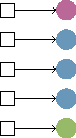
\includegraphics[]{figures/hash.pdf}
  \caption{\label{fig:hash} La clase \texttt{Lattice} contendrá una tabla hash en la que indexará los conceptos formales del retículo en base a su \textit{extent}.}
\end{figure}

\begin{notice}
  Hay que tener en cuenta que no podemos usar el número que en binario representa el \textit{extent} visto como un \texttt{bitset} ya que, para por ejemplo un contexto en el que consideremos 100 objetos, el número $2^{100}$ no puede ser almanceando en un \texttt{int}. Y tomar otra aproximación como \texttt{long long int} no creo que sea una solución adecuada, ya que seguiríamos estando limitados.
\end{notice}

\begin{idea}
  Sería iteresante implementar un \texttt{Lattice::iterator} el cual recorriese el retículo, no solo por un orden usual para recorrer grafos, como puede ser el preorden, sino también un orden marcado por una medida de bondad de conceptos formales. Ya vimos en el TFM que existían varias \textit{interestingness measures} para conceptos formales. También puede ser una medida que venga definida por el usuario, en base a sus preferencias para construir una descripción de la escena.
\end{idea}
Con esto vamos a comenzar a trabajar en el issue \issue{1}.

\entry{21/03/2020}

Hoy seguimos trabajando en el issue \issue{1}, dentro del objetivo \goal{1}, para ello vamos a proseguir con el trabajo sobre las clases \texttt{Lattice} y \texttt{Node}. Hay que tener algo en cuenta y es que ahora mismo estamos trabajando con un tamaño máximo para los \texttt{bitsets}, y por tanto para los contextos considerados \texttt{const int TMAX = 100;}, es decir, sólo podemos considerar contextos de una dimensión $100 \times 100$.

\begin{notice}
  Evidentemente podemos aumentar el tamaño de \texttt{TMAX} pero esto tiene un efecto sobre el tiempo de ejecución del programa, y no tiene que ver únicamente con el tamaño del contexto en sí. Si trabajamos con un contexto $100 \times 100$, pero empleando un \texttt{bitset<200>} veremos cómo el tiempo de ejecución de la aplicación aumenta. Es decir, el tamaño de las operaciones con \texttt{bitsets} de mayor tamaño es más costosa que para \texttt{bitsets} más pequeños. Con lo cual emplear el tamaño adecuado de \texttt{bitset} es importante. Esto da lugar al issue \issue{2}.
\end{notice}

Lo que hemos hecho para implementar la tabla hash es usar un \texttt{std::unordered\_map} que como clave tendrá un \texttt{string}, aprovechando el método \texttt{bitset::to\_string}.
\begin{lstlisting}

\end{lstlisting}

\appendix

\section{Objetivos y Análisis de Requisitos}
\label{sec:objetivos-requisitos}

\subsection{Objetivos}

\begin{itemize}
  \item[O1] Obtener el retículo de conceptos correspondiente a un contexto formal.
  \item[O2] Definir distintas medidas de bondad para las \textit{referring expressions} obtenidas.
  \item[O3] Refinamiento mediante propiedades contextuales.
\end{itemize}

\subsection{Análisis de Requisitos}
\label{sec:requisitos}

\begin{itemize}
  \item[r1] Permitir trabajar con la estructura de grafo que representa el retículo de conceptos formales de un contexto formal. Relacionado con el objetivo O1.
\end{itemize}

\subsection{Diagramas de Casos de Uso}
\label{sec:casos-uso}

\section{Diagrama de Clases}
\label{sec:clases}

\begin{center}
  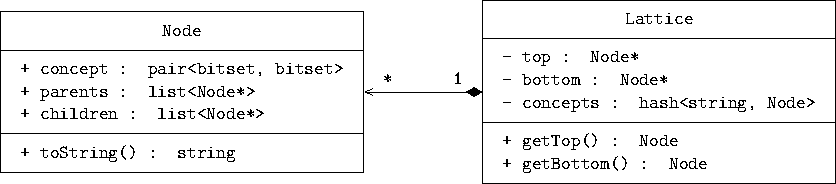
\includegraphics{figures/diagram.pdf}
\end{center}

\end{document}

%%% Local Variables:
%%% mode: latex
%%% TeX-master: t
%%% End:
